\documentclass[12pt]{report}
\usepackage[a4paper,
bindingoffset=0.2in,
left=0.1in,
right=0.1in,
top=0.5in,
bottom=0.5in,
footskip=.25in]{geometry}
\usepackage[utf8]{inputenc}
\usepackage[english]{babel}
\usepackage[myheadings]{fullpage}
\usepackage[T1]{fontenc}
\usepackage{fancyhdr}
\usepackage{graphicx, setspace}
\usepackage{sectsty}
\usepackage{url}
\usepackage{pdfpages}
\usepackage{subcaption}
\usepackage{amsmath}
\usepackage{multirow}
\usepackage{tikz}
\usepackage{minted}
\usepackage{hyperref}
\usepackage{amsfonts}
\usepackage{bbm, dsfont}
\usepackage{tikz}
\usepackage{mathtools}
\usepackage{csquotes}
%\usetikzlibrary{positioning}
\usetikzlibrary{shapes,positioning,calc,quotes}
\tikzstyle{subrotina} = [rectangle, draw,text centered, minimum width=5em, inner sep=5pt]
\tikzstyle{funcao} = [rounded rectangle, draw, text centered, minimum width=7em, inner sep=5pt]
\tikzstyle{random} = [rectangle, text centered, inner sep=5pt, minimum width=5em]
\tikzstyle{loop} = [rectangle, draw, align=left]
\tikzstyle{fluxo} = [draw, thick, -latex]
\tikzstyle{meiofluxo} = [draw, -]
\tikzstyle{chamada} = [draw, dashed, <->]


%%------ 
%% Comandos gerais
%% Observação: o arquivo "comandos.tex" tem que estar presente.
%%------
\input{comandos}
%%-----
%% Página de título
%% Observação: As definições que aparecem a seguir comporão a
%%             página de título e a folha de rosto.
%%-----
%% Define o nome da universidade onde o projeto foi desenvolvido.
\universidade{Universidade de São Paulo}
%
%% Define o nome da faculdade onde o projeto foi desenvolvido.
\faculdade{Instituto de Ciências Matemáticas e de Computação (ICMC)}
%
%% Define o título do projeto.
\titulo{Asymptotics of partition functions in random matrix theory}
%
%% Define a agencia de Fomento e a abreviatura. O primeiro argumento é o 
%% nome por extenso e o segundo a abreviatura.
%% Ambos os argumentos são obrigatórios
\agFomento{Fundação de Amparo à Pesquisa do Estado de São Paulo}{FAPESP}
%
%% Define o tipo de relatório. Pode ser Anual ou Final.
%% Não é obrigatório definir o tipo de relatório.
\tipoRelatorio{Anual}
%
%% Define a modalidade de Projeto. Pode ser temático, regular, etc.
\modalidadeProjeto{Masters }
%
%% Define o número do projeto.
%% Não é obrigatório definir o número do projeto.
\numProjeto{2024/06997-1} 
%
%% Define o autor do relatório.
\autor{Guilherme L. F. Silva}
%
%% Define a equipe do projeto (incluindo o pesquisador responsável no comando \membroA{}
\membroA{Guilherme L. F. Silva}
%% Inclua os demais membros do grupo (máximo +5)
\membroB{João Victor Alcantara Pimenta}
%\membroC{Francisco}
%\membroD{Joao}
%\membroE{Antonio}
%\membroF{José}
%
%% Define o período da vigência do Projeto.
\periodoRelatorio{20/04/2025 a 20/03/2026}
%
%% Define o período coberto pelo relatório.
\periodoVigencia{01/08/2024 a 31/07/2026}
%
%% Define a cidade onde o projeto foi desenvolvido.
\cidade{São Carlos}

%%-----
%% Página de título
%% Observação: Os comandos a seguir não devem ser mudados, 
%%             exceto caso necessário.
%%-----
\begin{document}
%
%% Define a numeração em romanos.
\pagenumbering{roman}
%
%% Gera a folha de título.
\geraTitulo
%
%% Gera a folha de rosto.
\folhaDeRosto
%
%% Escreva aqui o resumo em português.
\Resumo{
	The theory of Random Matrices finds its way in a diverse range of areas of Mathematics and Physics, and in particular to statistical mechanics. In the study of the spectra of eigenvalues of some random matrices ensembles, a physical analogy regarding thermodynamical systems becomes evident and the use of physical motivations in its study is of great importance. An example of such motivation is the study of the partition function, which holds in thermodynamics a great deal of information on the system at hand. Recent developments have been intensely unraveling new critical phenomena in random matrix theory, through a deep understanding of asymptotic expansions of the associated partition functions in the thermodynamic limit. The main goal of this work is to understand these developments in the context of normal random matrices, their relevance and implications in the theory of random matrices and beyond. 
 %Random Matrices can be though of in two ways: As a measurable function from a probability space into a set of matrices or, more concretely, as a matrix whose entries are random variables with some joint distribution. A set of such matrices with a given arbitrary distribution is called an ensemble. One can, for ensembles of interest, study statistic such as the eigenvectors and eigenvalue distributions. The symmetries of chosen set will reflect on what models such statistics can model. For example, distances of the characteristic values of a symmetric matrix with random coefficients model distances between successive levels of energies of heavy nuclei. More interestingly, there is some universality in the statistics found among classes of ensembles, suggesting the relevance of the theory in studying the universality in general modeled phenomena. Particularly important is the study of such matrices when they grow infinitely large, taking asymptotically its statistical behavior. We focus on a technique for deriving asymptotics for the so-called partition function of some interesting ensembles of random matrices.
  }
%
%% Escreva aqui o resumo em inglês.
% \Abstract{
%	The study of Random Matrices demonstrates applicability in a diverse range of areas, empha-
%	sizing the study of statistical mechanics, mainly in the simulation of gases. By studying the
%	spectral density of Gaussian matrix systems, one can develop the simulation of Coulomb gas
%	systems in analogy. Some difficulties arise in implementing simulations based on this theory,
%	mainly in system scalability and the treatment of possible singularities. To solve these pro-
%	blems, the literature has simulated these gases, with excellent numerical behavior, using the
%	Monte Carlo Hybrid Algorithm. We wish to explore this problem, the simulations, and the
%	proposed algorithm along with extending the potentials to wich it has been tested.
%}
%
%% Adicionará o sumário.
%% Mantenha o \thispagestyle{empty} e \clearpage
\tableofcontents
\thispagestyle{empty}
\clearpage
%
%% Define a numeração em arábicos.
\pagenumbering{arabic}

%%-----
%% Formatação do título da seção
%%-----
\sectionfont{\scshape}

%%-----
%% Corpo do texto
%%-----

\chapter{Period Achievements}\label{chp:realizacoes}

\section{Developed Activities}
\label{section:atividadesdesenvolvidas}

The following list summarizes the activities for the months covered by the report.

\begin{enumerate}
	\item \textbf{Completion of the Courses Necessary Credits}: It was completed  - in the second semester of 2025 - the necessary courses to fulfill the credits requirements for the Masters course in the Institution;
	
	\item \textbf{Publication of papers}: in the time covered by this report two papers were published were the process beneficiary is a co-author.	\enquote{A Central Limit Theorem for intransitive dice} published in \textit{ALEA, Lat. Am. J. Probab. Math. Stat. (v22-46)}, 2025, with DOI 10.30757. 	\enquote{Simulating Simple Random Walks With a Deck of Cards} published in \textit{Brazilian Journal of Probability and Statistics (25-BJPS635)}, 2025, with DOI 10.1214.
	
	\item \textbf{Participation in Events}: Many events have been attended in the period covered by this report. It was presented a poster \eqref{App: CLAPEM} at CLAPEM - Latin American Congress of Probability and Mathematical Statistics held in Montevideo - Uruguay in March, 2026. Money from the research found was used to take part in this event.  A poster \eqref{App: WTD} was also presented at the \enquote{XV Workshop de Teses e Dissertações em Matemática} held in São Carlos - Brazil in October, 2025. He took part in the \enquote{Fourier Analysis \& Beyond I} held in IMPA, Rio de Janeiro from June 30th to July 04th, 2025. He also took part in the \enquote{35º Colóquio Brasileiro de Matemática} held IMPA, Rio de Janeiro from July 27th to August 1st, 2025. The student also took part in an extension project called SigmaCamp \url{https://sigmacamp.org/} - and international advanced scientific camp for young students. He took part in the ETAPA SigmaCAMP and the SigmaFestival where he taught classes on mathematical and physical subjects besides doing administrative tasks along a team of international researchers from all sciences and institutions.
	
	\item \textbf{Continuous study of theory and meaningful literature}: As the natural way to research, we gave continuation to the reading material in the theory and started focusing -  in the second semester of 2025 - in the main research article \cite{Byun_2023} we will work on the remaining months;
		
	\item \textbf{Masters Thesis}: It was begun the process of organizing and writing what will become the final product of the masters project, the thesis.
	
\end{enumerate}

\section{Schedule}


This M.D. research proposal started in August 2024 and is running for the usual time for the Masters Program, that is, 24 months. The project was originally divided for execution in the following schedule.

%\begin{table}[ht]
%\centering
%\begin{tabular}{|c|c|c|c|c|c|c|c|c|c|c|c|c|}
%\hline
%\multirow{2}{*}{{\bf Fases}} & \multicolumn{6}{c|}{{\bf Meses}}
%\\ \cline{2-7}
%    & 1 & 2 & 3 & 4 & 5 & 6
%\\ \hline
%    {\bf 1. Revisão Literatura RMT} & x & x & x & & &  
%\\ \hline
%    {\bf 2. Métodos de Simulação} &  &  & x & x & &
%\\ \hline
%    {\bf 3. Implementação algoritmos} & & & & x & x & 
%\\ \hline
%    {\bf 4. Redação Relatórios} & & & & & & x
%\\ \hline
%\end{tabular}
%\caption{Cronograma das atividades.}
%\label{tab:cronograma6meses}
%\end{table}
\begin{table}[ht]
	\centering
	\begin{tabular}{|c|c|c|c|c|c|c|c|c|c|c|c|c|}
		\hline
		\multirow{2}{*}{{\bf Steps}} & \multicolumn{8}{c|}{{\bf Quarters}}
		\\ \cline{2-9}
		& 1 & 2 & 3 & 4 & 5 & 6 & 7 & 8
		\\ \hline
		{\bf 1. Master Courses} & \textcolor{green}{x} & \textcolor{green}{x} & \textcolor{green}{x} & \textcolor{green}{x} & \textcolor{green}{x}  & \textcolor{green}{x}  & & 
		\\ \hline
		{\bf 2. Concepts} &  &  & \textcolor{green}{x}  & \textcolor{green}{x}  & \textcolor{green}{x} & \textcolor{green}{x}  & &
		\\ \hline
		{\bf 3. Main Article} & & & & \textcolor{green}{x}  & \textcolor{green}{x}  & \textcolor{green}{x} & x &
		\\ \hline
		{\bf 4. Exploration} & & & & & \textcolor{green}{x} & \textcolor{green}{x} & \textcolor{red}{x} & 
		\\ \hline
		{\bf 5. Masther Thesis} & & & & & \textcolor{green}{x}  & \textcolor{green}{x} & \textcolor{red}{x} & \textcolor{red}{x}
		\\ \hline
	\end{tabular}
	\caption{Activities originally planned. Red color indicates the focus of the quarter that may be divided between activities. Green indicates the planning was accomplished.}
	\label{tab:cronograma1ano}
\end{table}

Naturally then, until the end of the project the student should be finalizing the study of the main article and writing the final thesis as he explores the possibilities of the research.

\section{Masters Courses}

During the Masters the student took part in the following courses.
\hspace{1cm}

\begin{center}
	\begin{tabular}{|c|c|c|c|}
		\hline
		\textbf{Course} & \textbf{Code} & \textbf{Concept} & \textbf{Semester} \\
		\hline
		Variedades Diferenciáveis & SMA5781-21/3 & A & 2 - 2024 \\
		\hline
	    Equações Diferenciais Ordinárias & SMA5802-17/2 & B & 2 - 2024 \\
		\hline
		Algebra& SMA5738-17/4 & A & 1 - 2025 \\
		\hline
		Medida e Integração & SMA5801-13/4 & C & 1 - 2025 \\
		\hline
		Introdução a Mecânica Celeste& SMA5998-1/1 & A & 2 - 2025 \\
		\hline
		Preparação Pedagógica& SMA5839-19/8 & A & 2 - 2025 \\
		\hline
	    Treinamento Profissional e Acadêmico & SMA5976-2/1 & A & 2 - 2025 \\
		\hline
	\end{tabular}
\end{center}

\section{Research Overview}
\label{Pesquisa}

Random Matrices can be though of in two ways: As a measurable function from a probability space into a set of matrices or, more concretely, as a matrix whose entries are random variables with some joint distribution. In some cases there is an explicit density formula for the eigenvalues of such a random matrix. For some Random Matrices, with the help of some mathematical tools such as orthogonal polynomials one can expresses the equilibrium measures for the eigenvalues asymptotically.  There are many instances of \enquote{models} of random matrices, each one with its symmetries and own probability density. Those are what we call \textit{ensembles}. 

Borrowing some concepts from physics, an ensemble can be though as a virtual collection of all possible states that a system can be in, with more probable states appearing more often in the collection. There is a analogy to be made with ensembles of thermodynamic: When considering sets of matrices with equal probability - in some sense to be more clear soon - we get the Gibbs weight for the probability distribution as we would in the physical \textit{Canonical Ensemble}, thought of as a system of particles with constant temperature. More concretely, in the context of Random Matrix Theory, we have the definition.

\begin{definition}
	A random matrix ensemble $\eE = (\eS, \eP)$ is a set of matrices $\eS$ of fixed size equipped with a probability density function (p.d.f.) $\eP: \eS \rightarrow [0, \infty)$. If we say that a matrix $\hat{X}$ is drawn from the random ensemble $\eE$, we are saying that it is a random variable assuming values in $\eS$ with p.d.f. $\eP$.
	\label{Def: Ensemble}
\end{definition}

In the research proposed here, we will focus on the study of {\it normal random matrices}, which consists of the space of normal matrices, equipped with a proper probability distribution. In the beginning of its book, Feynman states \cite{feynmanstatistical} that the key principle of the statistical mechanics is that the probability that a system attains a state with energy $E$, in equilibrium, is given by a function $\frac{1}{Z} \ee^{\frac{-E}{kT}}$ where $Z$ is the partition function. In a more general sense there is a relation between the partition function and the free energy of the system, that, in itself, relates to the entropy. Knowing well the partition function is a way to describe with great detail the macro-properties of such a system.

There is a great effort in the community of random matrix theory to study expansions of the partition function of various classes of Random Matrix. Recently, some advance has been made in the works of Sug-Soo Byun et al. \cite{Byun_2023}. The work they done was on Random Normal Matrix and Planar Ensembles (with Determinantal and Pfaffian structures, respectively), which present partition functions
\begin{equation}
	Z_N^{(\beta)} \deff \int_{\C^N}  \prod_{j>k=1}^{N} |z_j - z_k|^\beta \prod_{j=1}^{N} \ee^{-\frac{\beta N}{2} Q(z_j)} \dd A(z_j)
\end{equation}
where $N$ is the size of the matrix, $\beta$ is relative to the generic entries dimension and $\dd A(z) \deff \dd^2 z/\pi$ is the area measure. Here, $Q: \C \rightarrow \R$ is called the confining potential and satisfies some suitable conditions. In their work, using concepts of orthogonal polynomials and integral asymptotic by Laplace method, they derived large-$N$ asymptotic expansions up to the $O(1)$-terms for  $Z_{N,\beta}$ when $V$ is a radially symmetric potential, in the form
%
$$
Z_{N,\beta=2}=-I^VN^2+\frac{1}{2}N\log N+E^V N+G\log N+F^V + o(1),\quad N\to \infty.
$$
%
In such expansion, for a large class of potentials $V$ the first term $I^Q$ was known for a long time, being given by the energy of the associated equilibrium measure. The coefficient $1/2$ of the order $N\log N$, as well as the entropy term $E^V$, were known from recent work of Leblé and Serfaty \cite{Leble2017-yj}, also for rather large classes of $V$. The remaining terms in this expansion are new, and they are computed exploring the radially symmetry imposed on the potential. Strikingly, the term $G$ appears to be universal in $V$, depending solely on the connectivity of the limiting spectrum of eigenvalues. More precisely, they noticed that $G$ depends on whether the limiting spectrum is an annulus or a disc which, surprisingly, seems to not have been observed in the vast previous literature on the matter. 

As was said, the study of the partition function is a major way to describe thermodynamic systems. With these new developments it is expected that many systems could be better understood and described by the asymptotic given. In that way this poses a great opportunity for development in the field. More than that, by the great connection that the field of random matrices holds with many other fields is possible that by the study of this work some suggestions on the behavior of many other related problems become plausible. Especially, we will be interested in external field model.

\chapter{Scientific Events}\label{chp:particEvento}

Many events have been attended in the period covered by this report. It was presented a poster \eqref{App: CLAPEM} at \textbf{CLAPEM} - Latin American Congress of Probability and Mathematical Statistics held in Montevideo - Uruguay in March, 2026. Money from the research found was used to take part in this event.  A poster \eqref{App: WTD} was also presented at the \enquote{XV Workshop de Teses e Dissertações em Matemática} (\textbf{WPGMAT}) held in São Carlos - Brazil in October, 2025. He took part in the \enquote{Fourier Analysis \& Beyond I} (\textbf{FAB}) held in IMPA, Rio de Janeiro from June 30th to July 04th, 2025. He also took part in the \enquote{35º Colóquio Brasileiro de Matemática} (\textbf{CBM}) held IMPA, Rio de Janeiro from July 27th to August 1st, 2025. The student also took part in an extension project called SigmaCamp \url{https://sigmacamp.org/} - and international advanced scientific camp for young students. He took part in the ETAPA SigmaCAMP and the SigmaFestival where he taught classes on mathematical and physical subjects besides doing administrative tasks along a team of international researchers from all sciences and institutions.

\hspace{1cm}

\begin{center}
	\begin{tabular}{|c|c|c|c|c|c|}
		\hline
		Event &  Institution & Date & Modality & Presentation & Research founds \\
		\hline
			FAB & IMPA & 30/06-04/07/2025 & Presential & Participant& No \\
		\hline
			CMB & IMPA & 27/07-01/08/25 & Presential & Participant & No \\
		\hline
			WPGMAT & ICMC-USP & 01/08/2025 & Presential & Poster - Oral & No \\
		\hline
			CLAPEM & SLAPEM & 01-06/03/23 & Presential & Poster - Oral & Yes \\
		\hline
	\end{tabular}
\end{center}


\chapter{Other prepared or submitted works}

During the period covered by this report two papers were published. The first one was \enquote{A Central Limit Theorem for intransitive dice} \eqref{App: Dice}, published in ALEA, Lat. Am. J. Probab. Math. Stat, 2025, with DOI 10.30757. The second was \enquote{Simulating Simple Random Walks With a Deck of Cards} \eqref{App: Cards}, published in Brazilian Journal of Probability and Statistics, 2025, with DOI 10.1214. Both are presented in the Appendix.
%%-----
%% Referências bibliográficas
%%-----
\addcontentsline{toc}{chapter}{\bibname}
\bibliographystyle{abntex2-num}
\bibliography{bibliografia}

%%-----
%% Fim do documento
%%-----

%\appendix
%\chapter{Implementação Algoritmo}

%\inputminted[
%frame=lines,
%framesep=2mm,
%baselinestretch=1.2,
%bgcolor=white,
%fontsize=\footnotesize,
%linenos
%]{FORTRAN}{Assets/HKMC.f}

\appendix

\chapter{Poster Workshop}
\label{App: WTD}
Poster presented in the \enquote{XV Workshop de Teses e Dissertações em Matemática} in ICMC. São Carlos, Brazil. 2025.

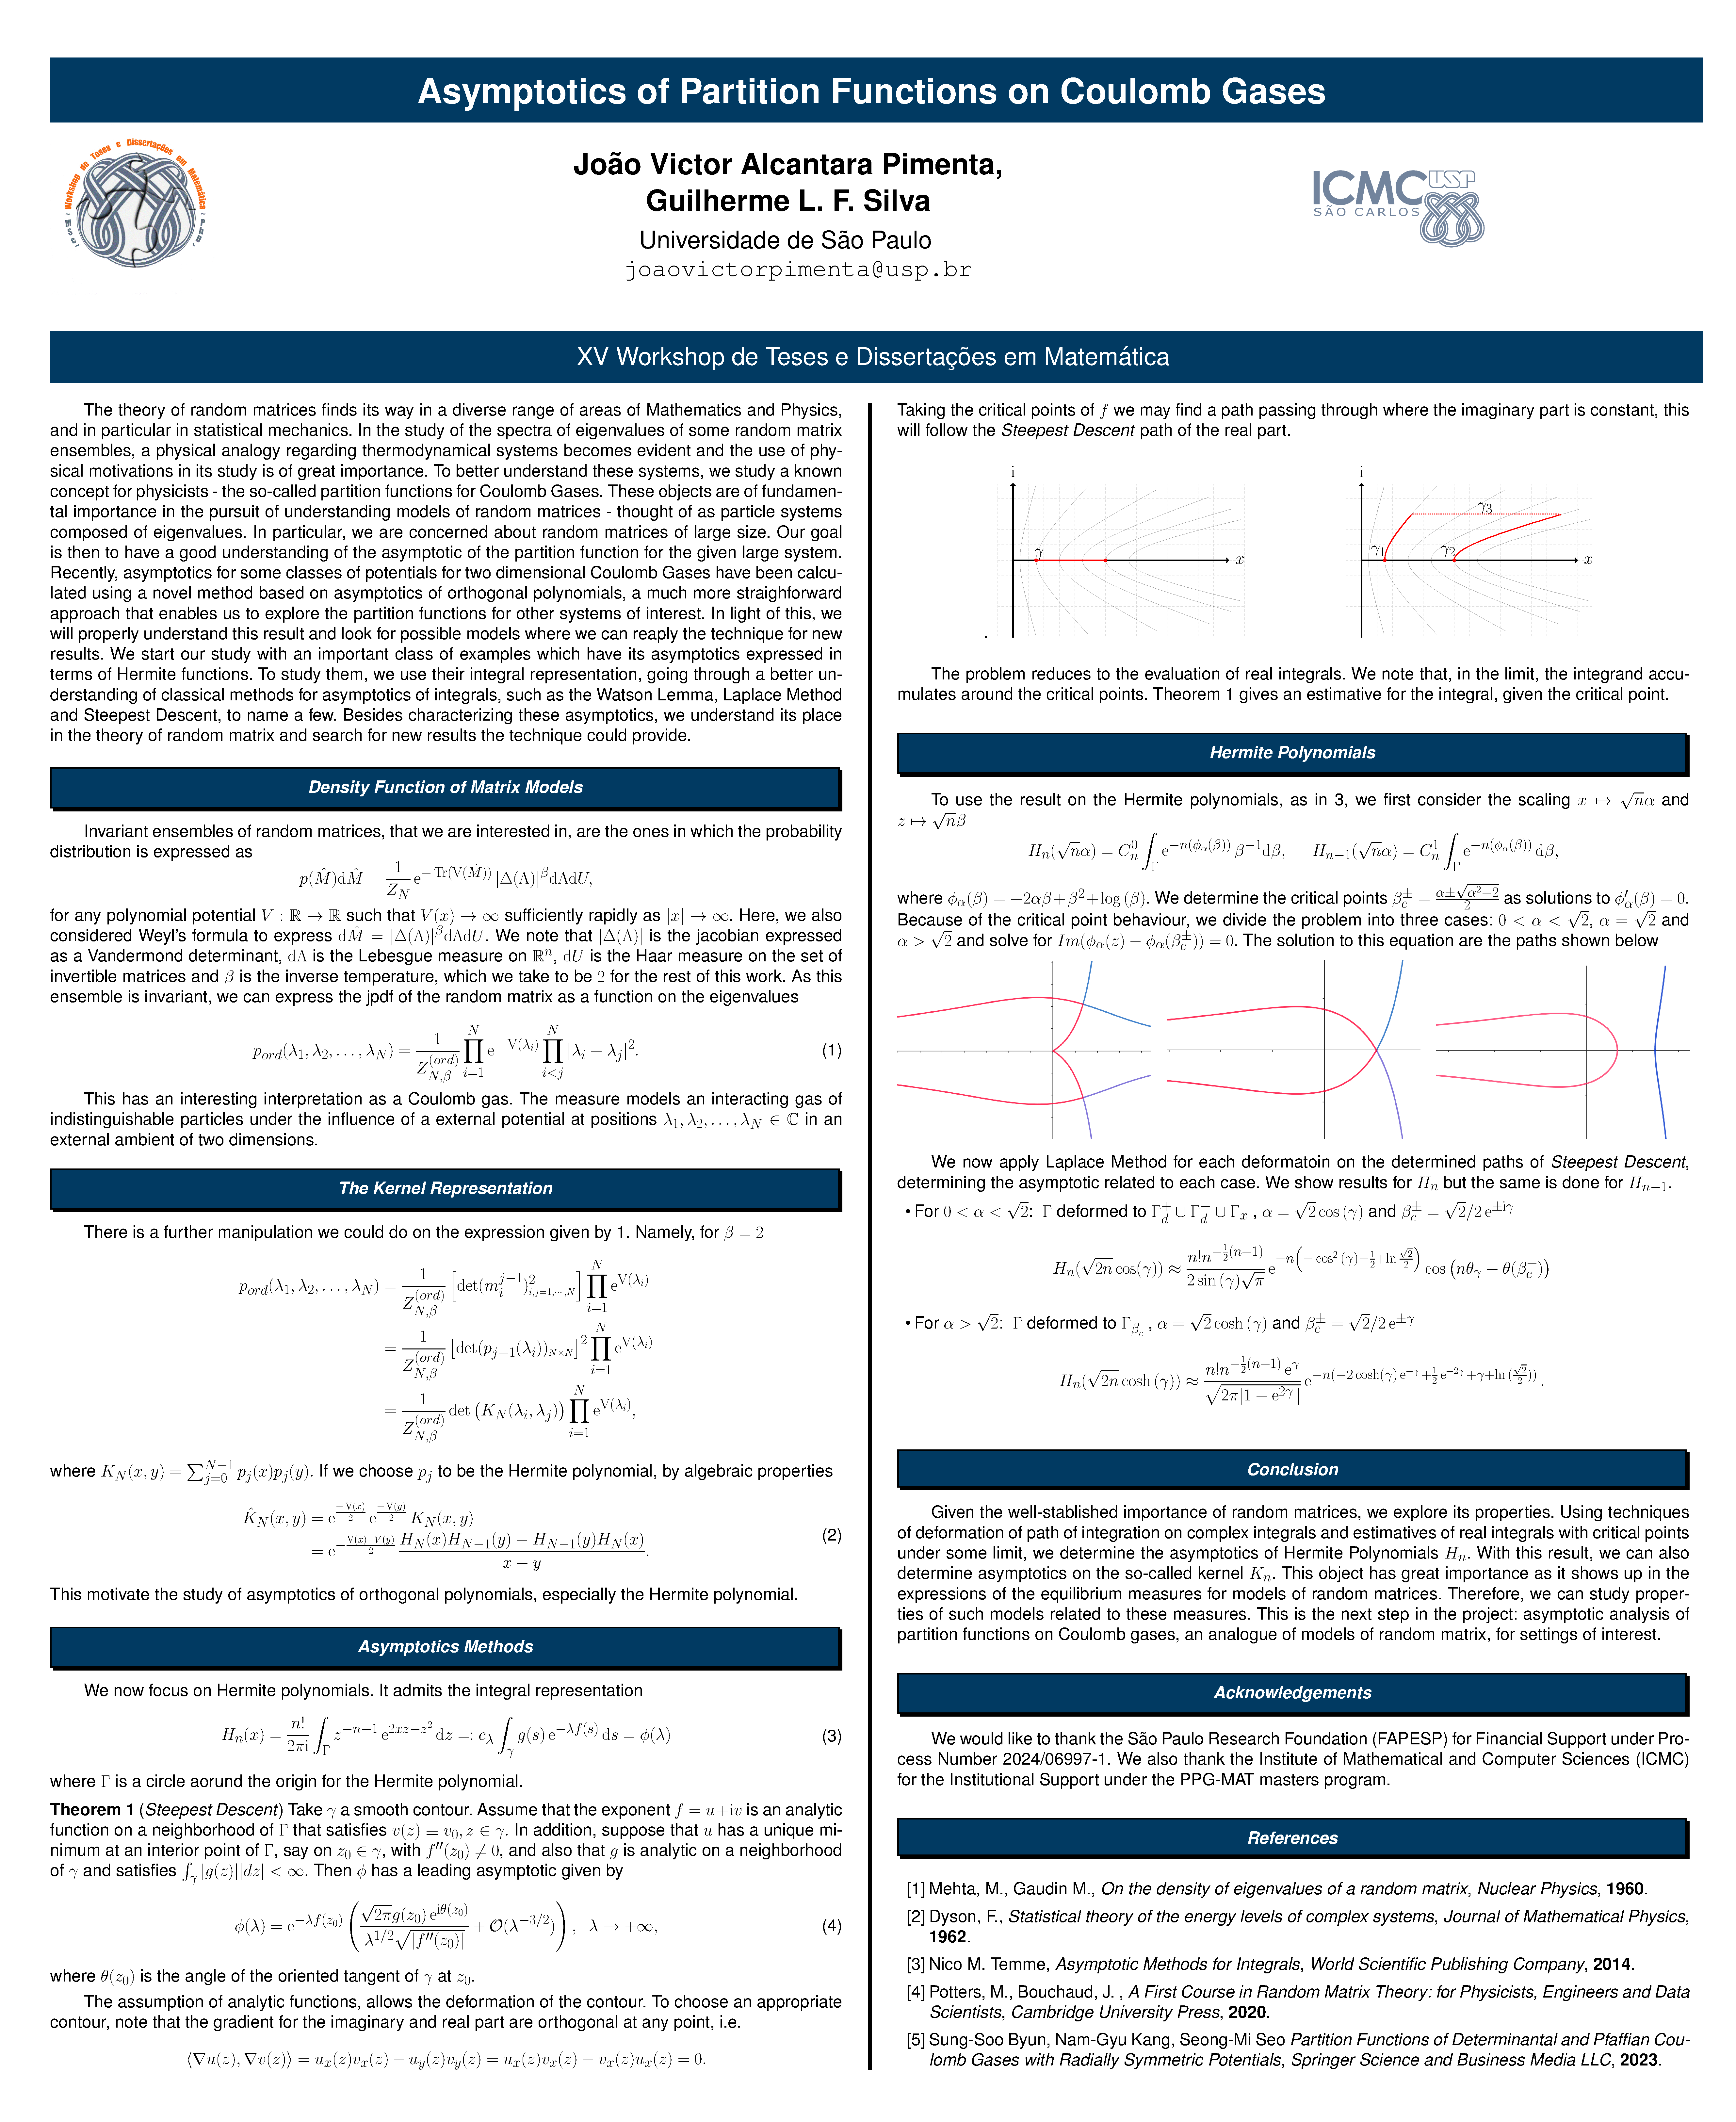
\includepdf[pages={1}]{Assets/WTD.pdf}

\chapter{Poster CLAPEM}
\label{App: CLAPEM}

Research Founds were used to take part in this event, because of that I declare that: This work was presented as a poster in the XVII CLAPEM - the Latin American Congress of Probability and Mathematical Statistics which has occurred on March 2-6, 2026 in Montevideo, Uruguay.


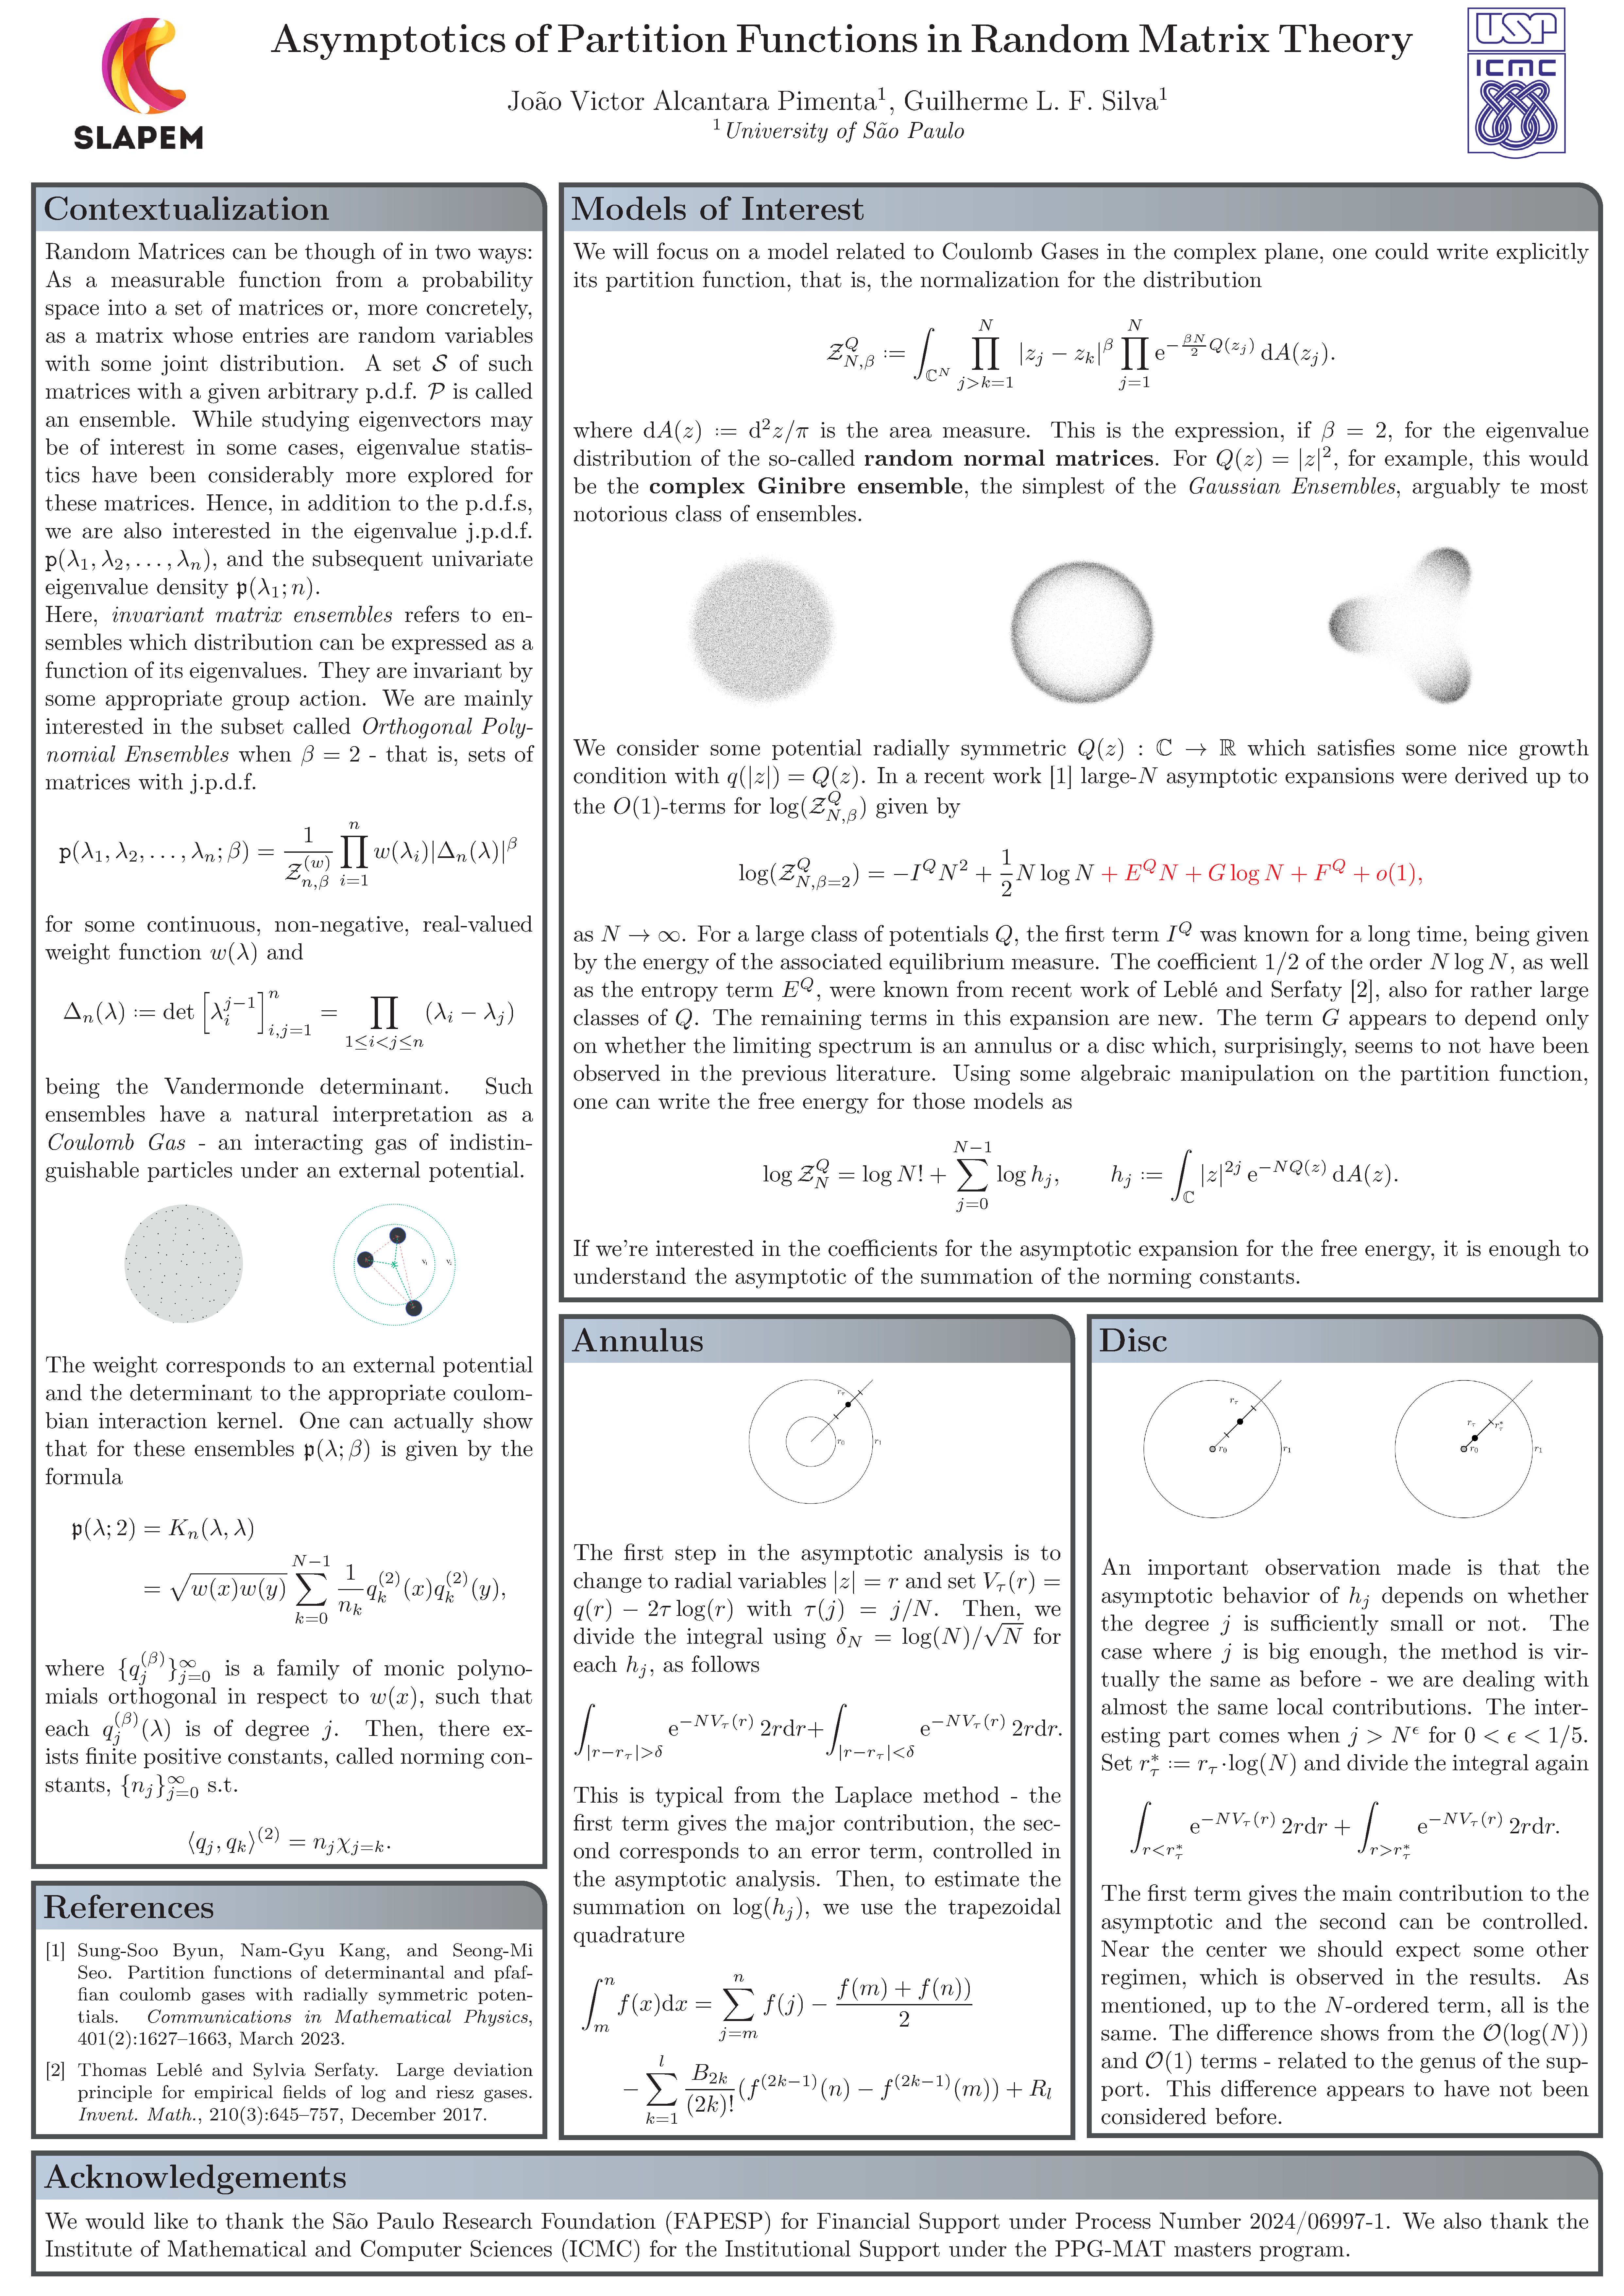
\includepdf[pages={1}]{Assets/CLAPEM.pdf}

\chapter{Paper: A Central Limit Theorem for intransitive dice}
\label{App: Dice}

Published Paper in \textit{ALEA}: \enquote{A Central Limit Theorem for intransitive dice}

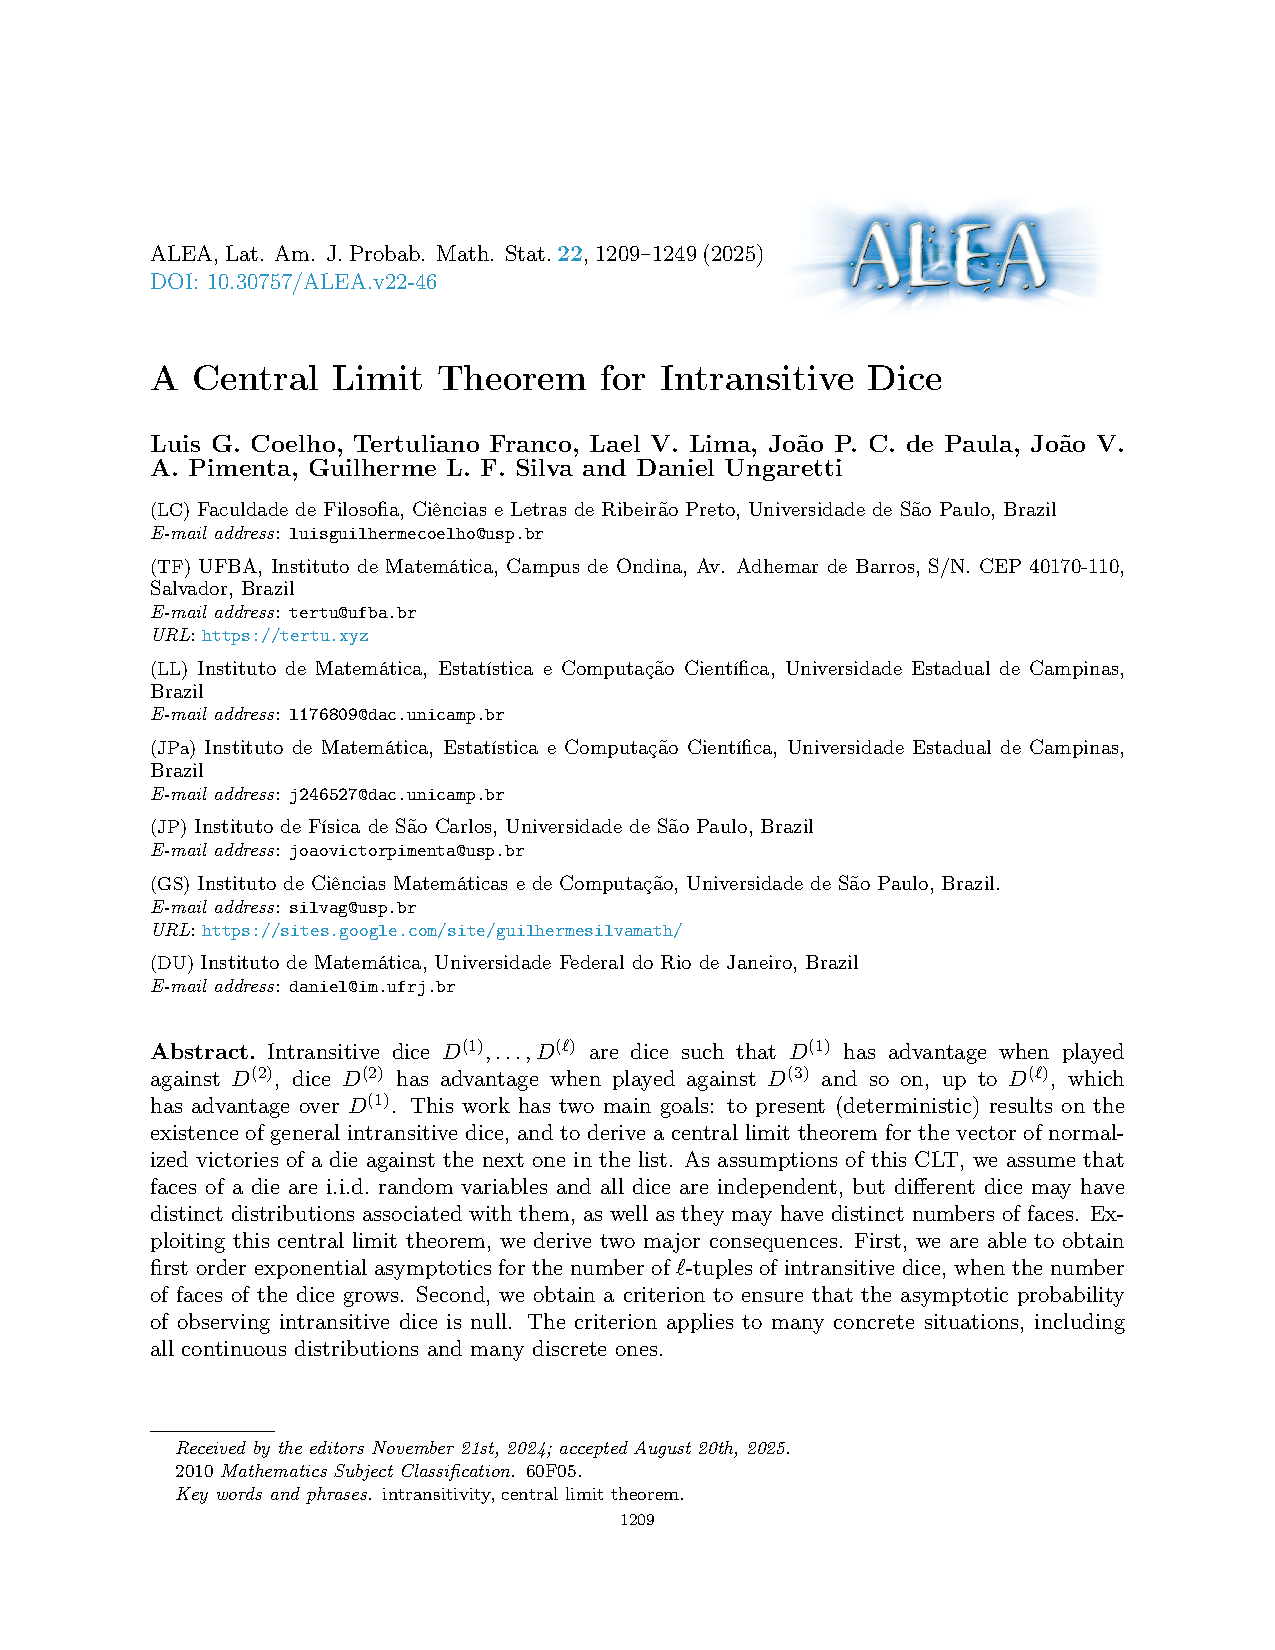
\includepdf[pages=1]{Assets/CLTID.pdf}

\chapter{Paper: Simulating Simple Random Walks With a Deck of Cards }
\label{App: Cards}

Published Paper in \textit{Brazilian Journal of Probability and Statistics}: \enquote{Simulating Simple Random Walks With a Deck of Cards}.

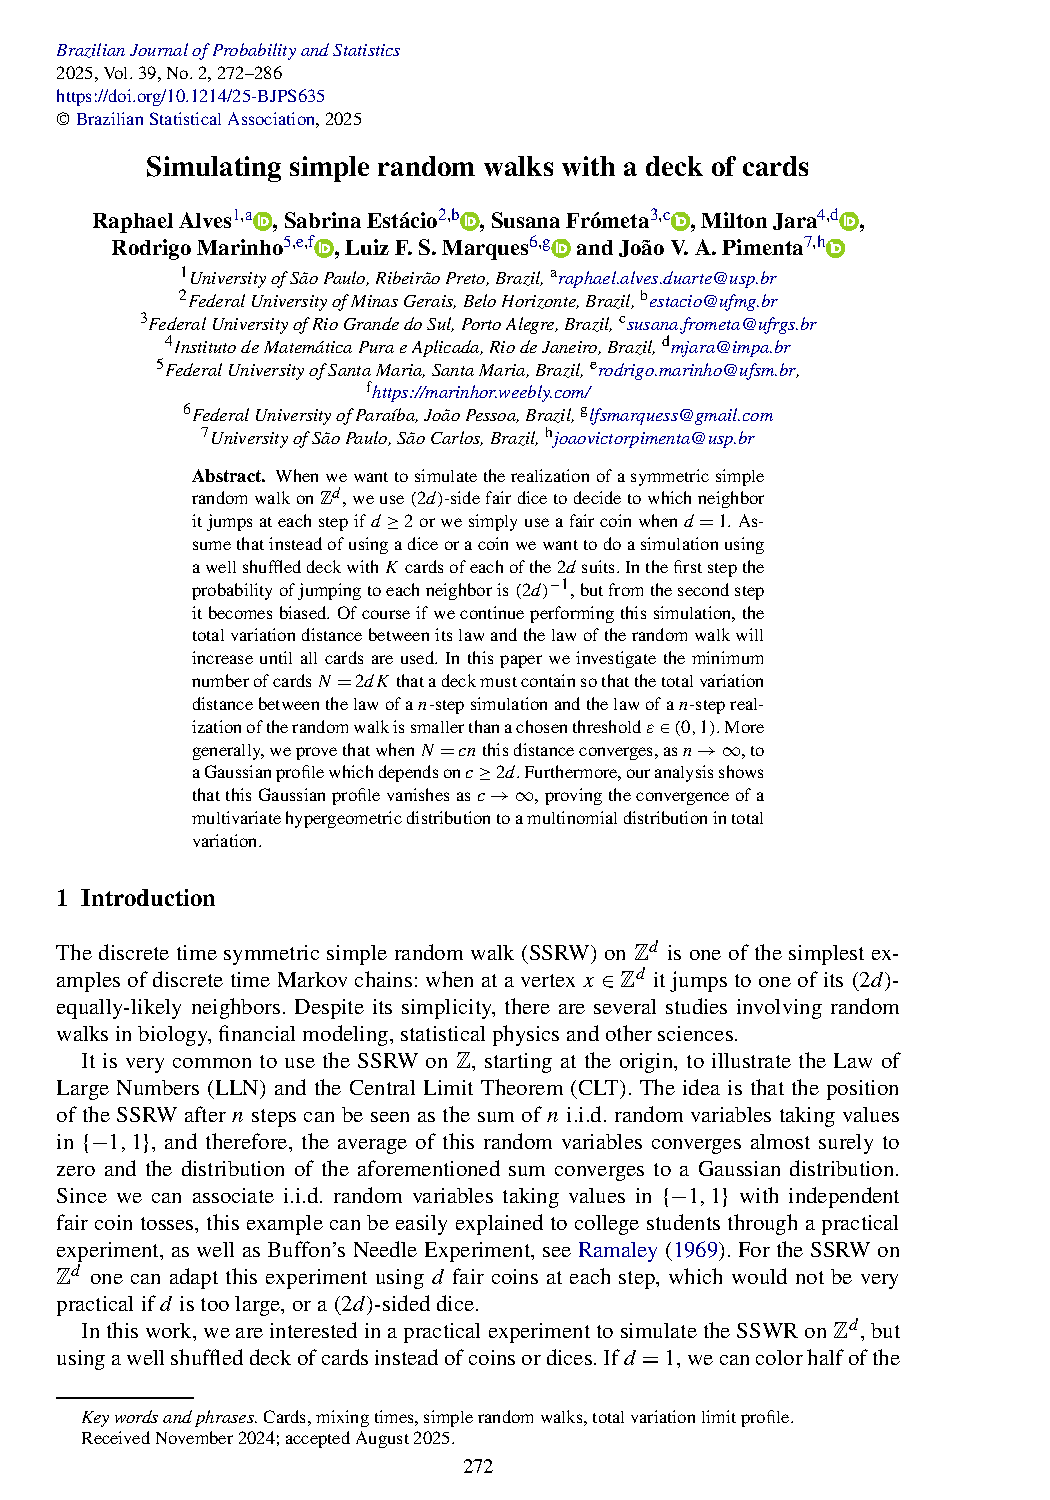
\includepdf[pages=1]{Assets/SSRWWDC.pdf}

\chapter{Student's Record}

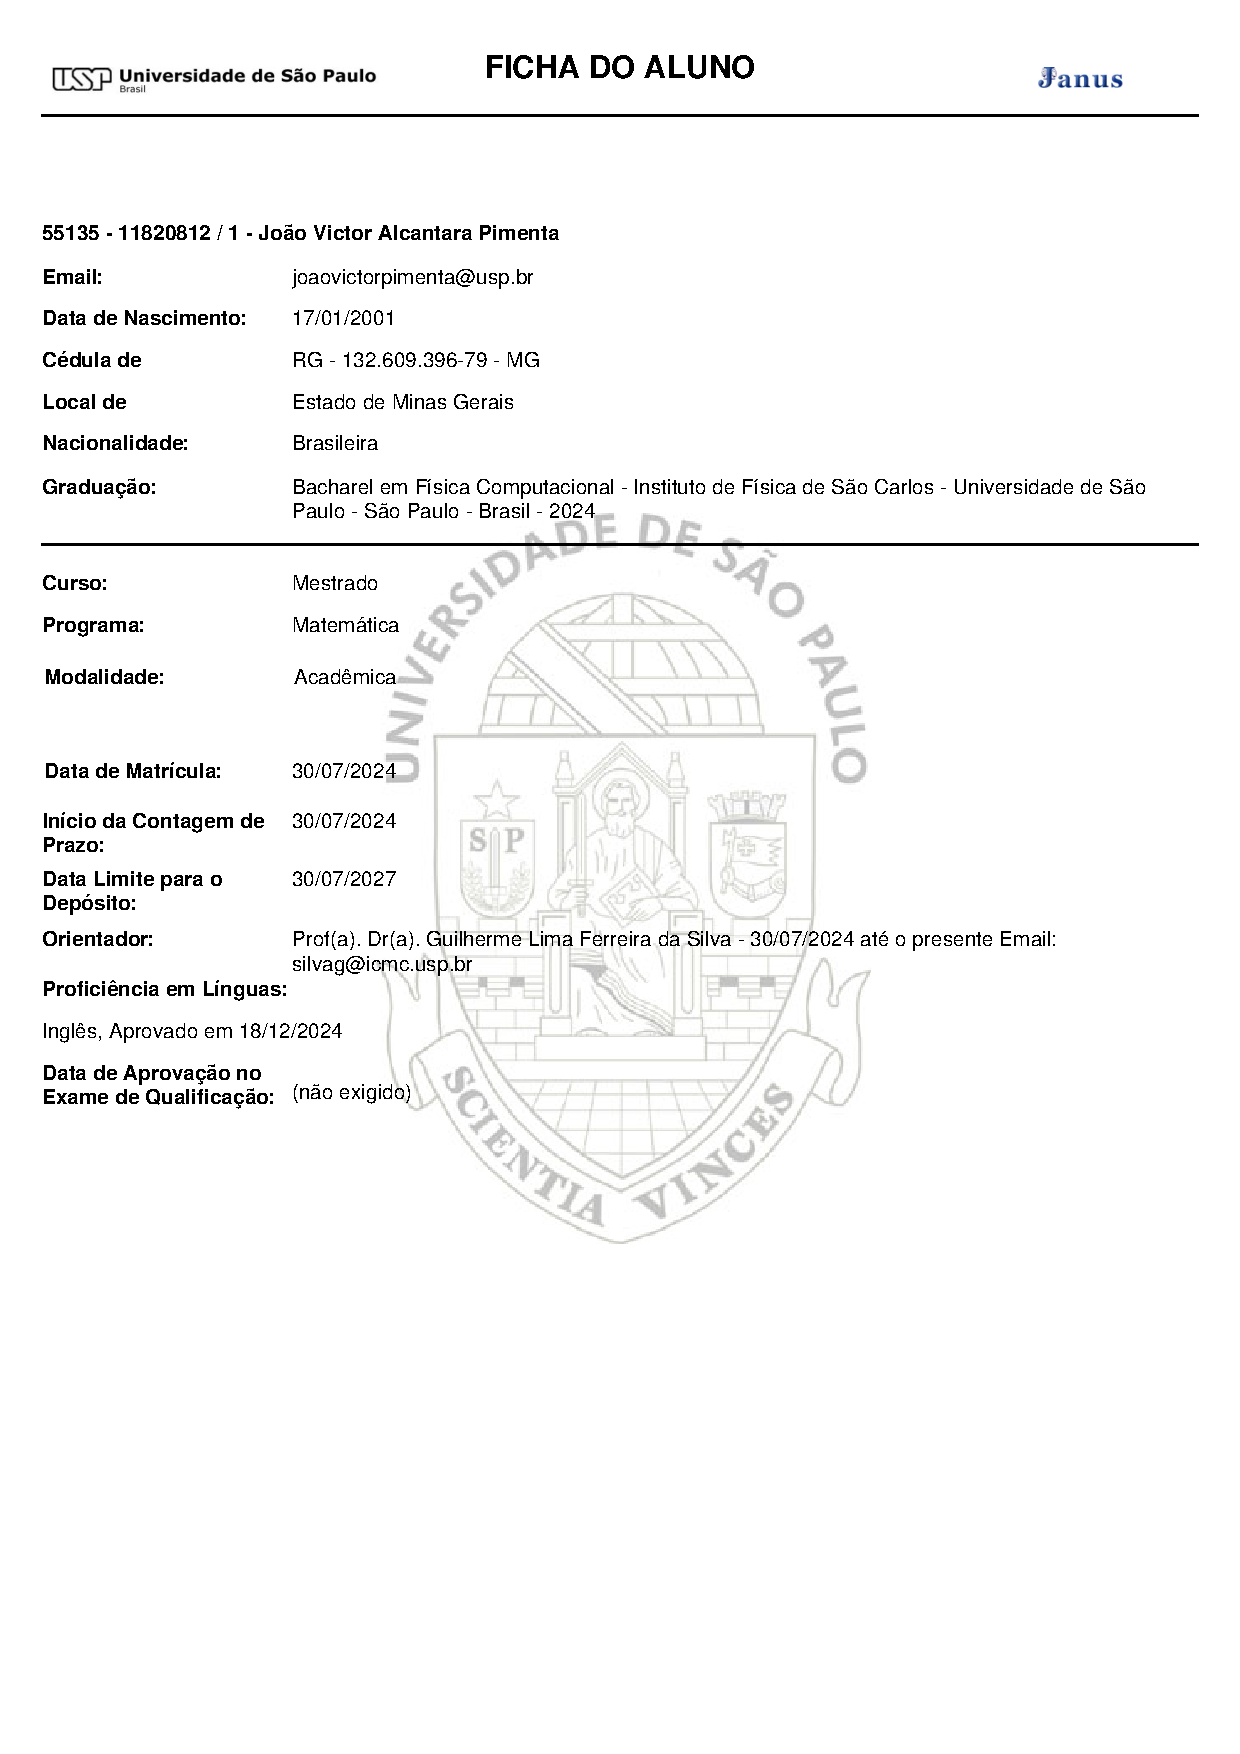
\includepdf[pages=1-3]{Assets/Record.pdf}

\end{document}